Before exploring the technical components of recognizing human emotions, it is exceedingly important to have a general idea about common emotion models and theories produced from psychology. Based on extensive research from leading psychologists, two models of emotional states emerged: Categorical and Dimensional. 

\subsection{Categorical Emotion Models}
    Categorical models are some of the most widely used models due to their ease of use and comprehendability. These models comprise a categories of independent emotions. Some of the most famous research dates includes Robert Plutchik's \cite{plutchik-2001} wheel of emotions shown in Figure \ref{fig:plutchik-wheel} containing eight distinct emotions: anger, anticipation, joy, trust, fear, surprise, sadness and disgust. The distance from the center of the wheel indicates intensity of the emotion and the proximity in the circle represents similarity among the emotions. Another renown psychologist, Paul Ekman, proposed that there are six basic emotions fear, anger, joy, sadness, disgust, and surprise \cite{ekman-1992}. 
    
    \begin{figure}[!htb]
    \centering
    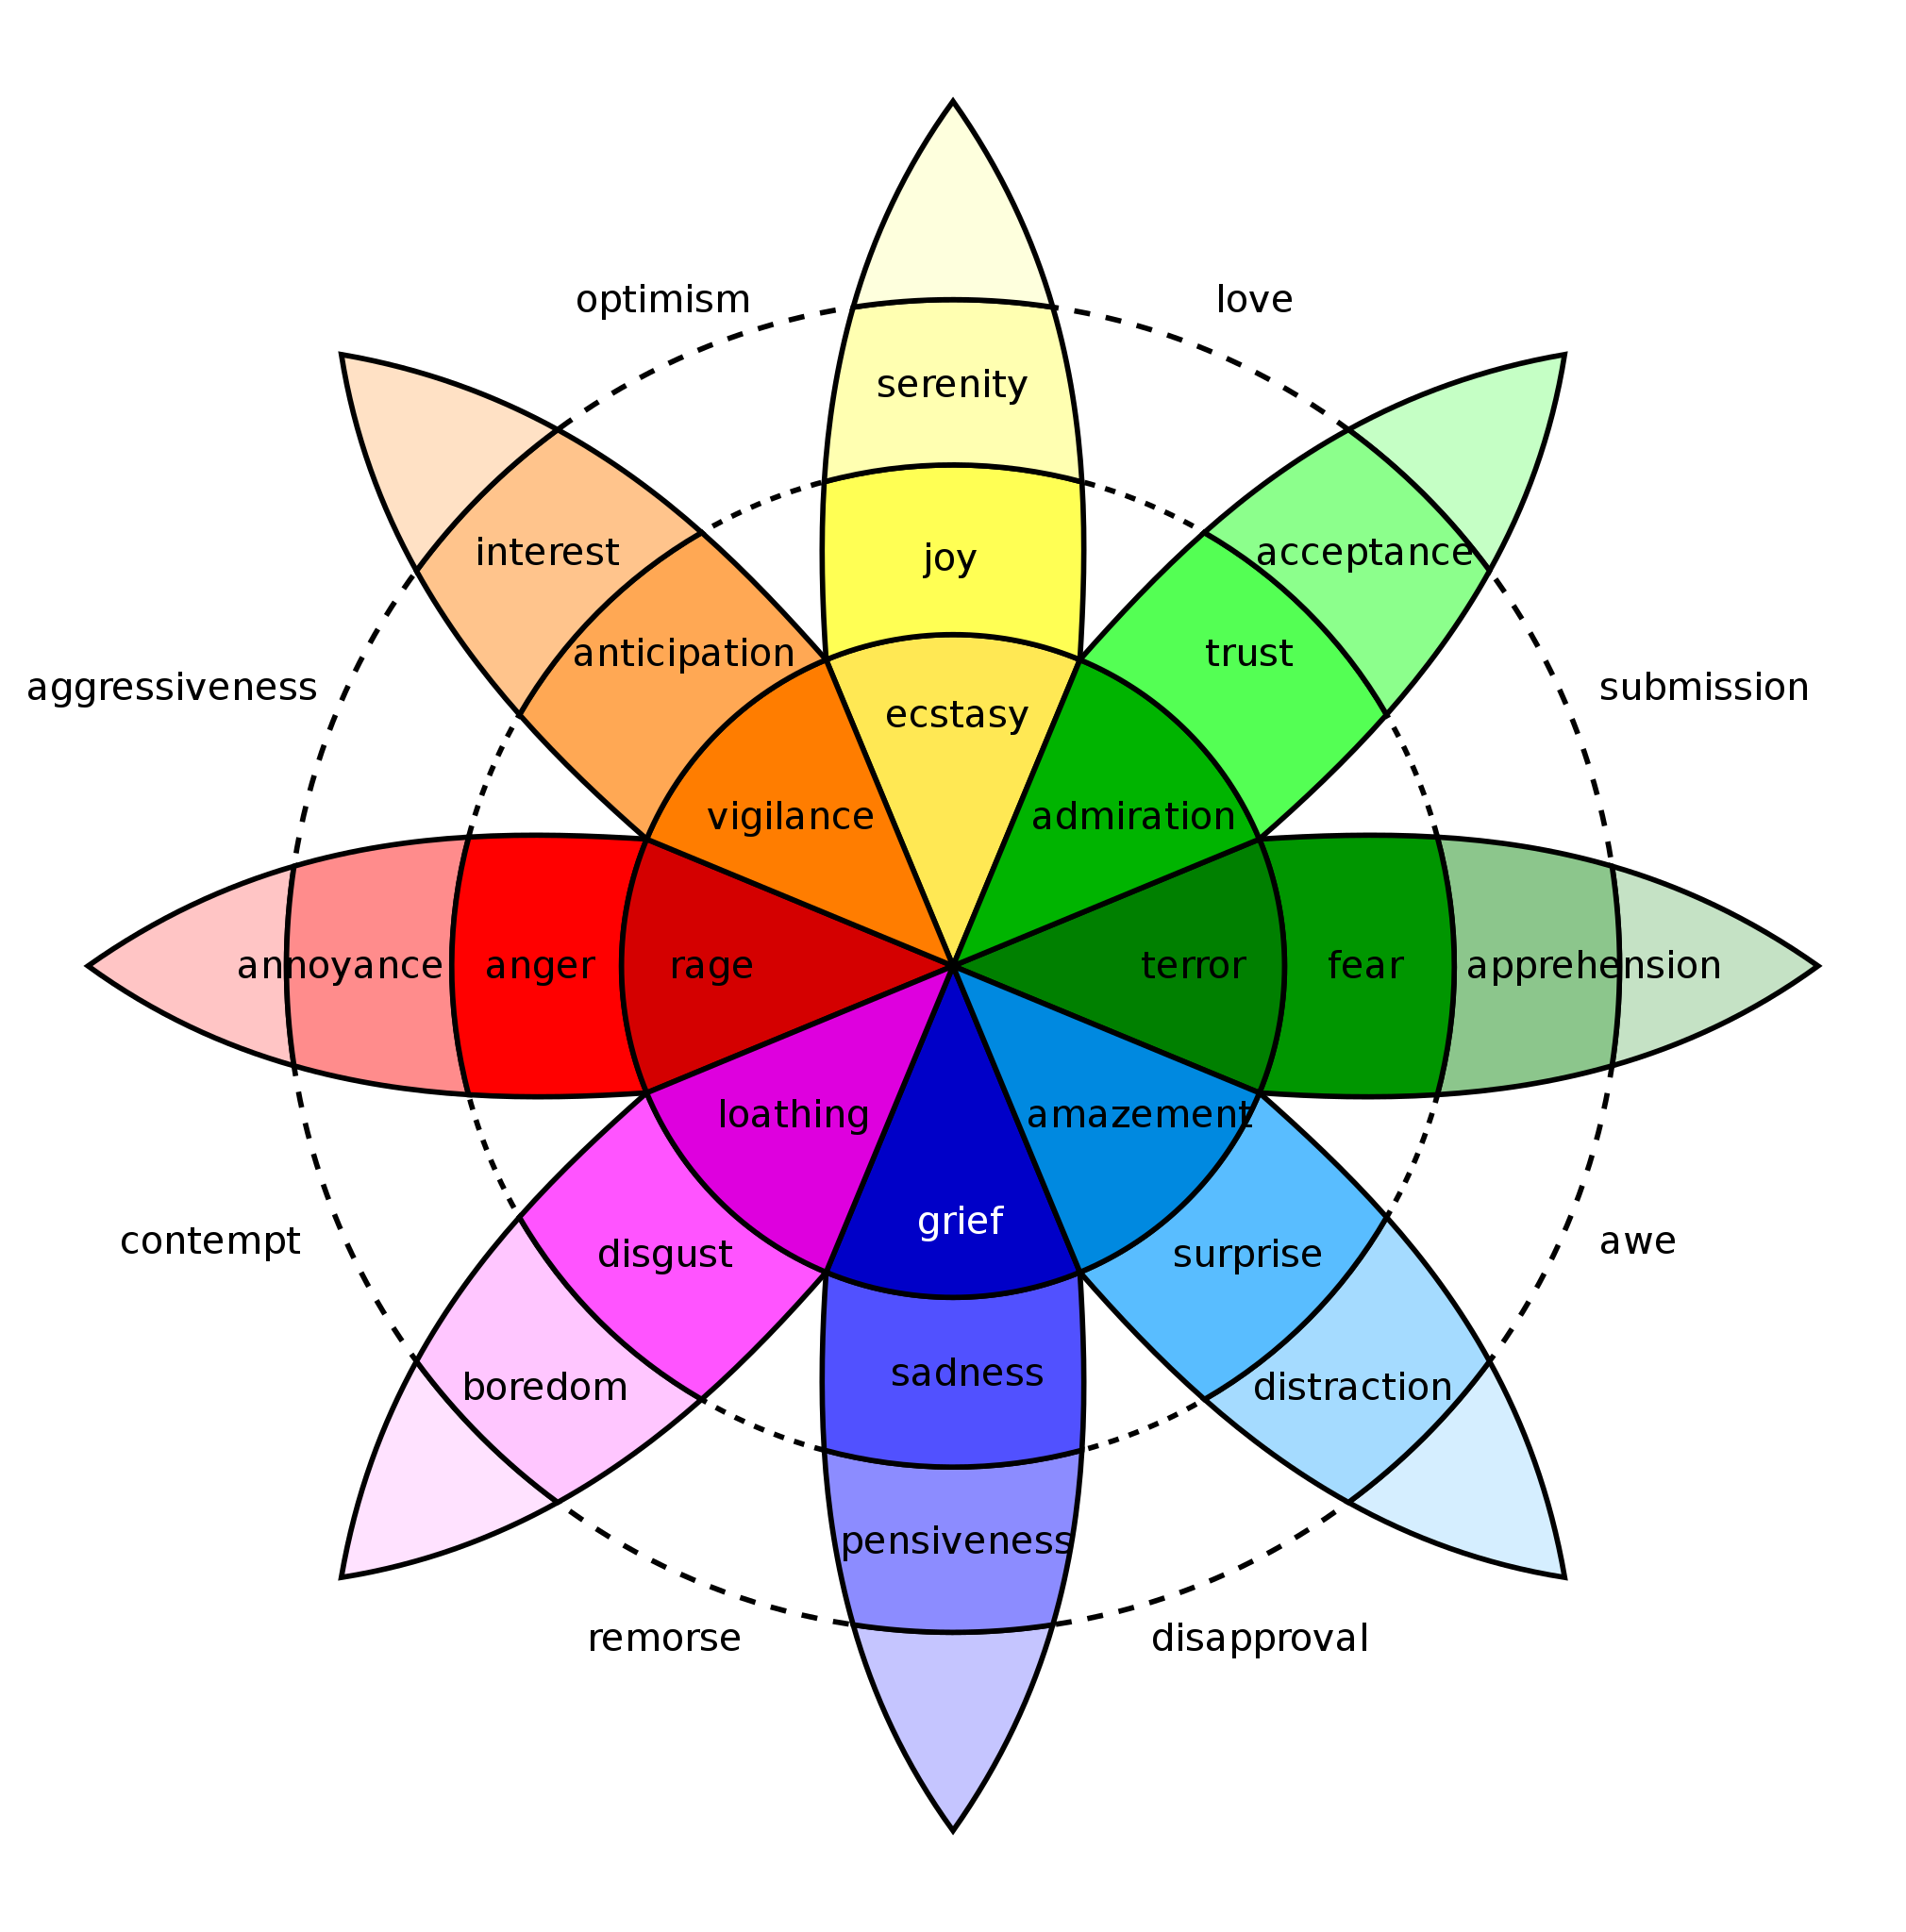
\includegraphics[width=.4\textwidth]{figures/Plutchik-wheel.png}
    \caption{\label{fig:plutchik-wheel} Plutchik Wheel of Emotions \cite{plutchik-2001}}
    \end{figure}
    
    Early emotion models are based on how humans express emotions using facial expressions. More recently, research findings proposed that disgust and anger share a similar wrinkled nose and fear and surprise share raised eyebrows\cite{jack-2014}. These differences in facial expressions are believed to be developed for social purposes and not as a basic emotion expression \cite{mansourian-2016}. Many other researchers \cite{gu-2016}\cite{gu-2019}\cite{zheng-2016} also agree with the model containing four basic human emotions: fear, anger, joy, and sadness. These four basic emotions are a subset of both foundational emotion models.

\subsection{Dimensional Emotion Models}
    Despite their ease of application, categorical models lack the ability to provide a continuous range of intensity to describe the depth of an emotion. As a result, two-dimensional models were developed to help explain the degree of emotion being expressed. Arguably the most famous 2D model was developed by James Russell, shown in Figure \ref{fig:russell}. In his model, he classifies emotions using arousal or alertness and valence (pleasure continuum). Using this model, each emotion can be explained by a simple combination of these two neurophysiological systems.
    
    \begin{figure}[!htb]
    \centering
    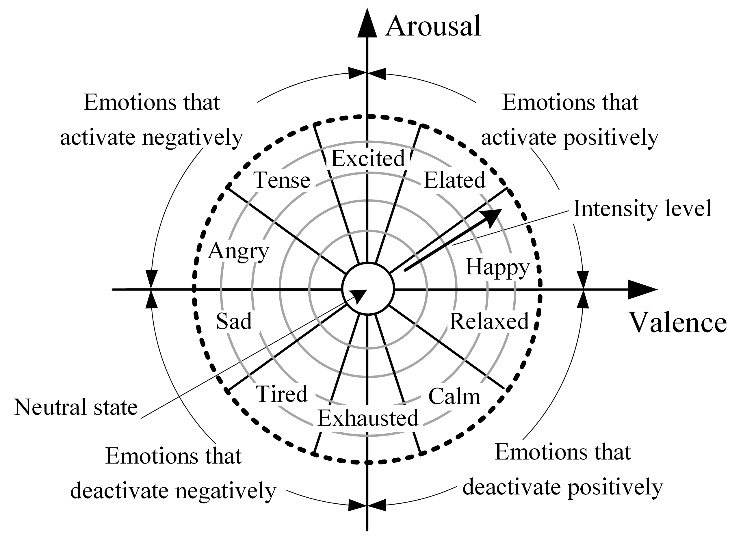
\includegraphics[width=.5\textwidth]{figures/russell_emotions.png}
    \caption{\label{fig:russell} Russell's Circumplex Model of Affect \cite{russell-nodate}}
    \end{figure}
    